\documentclass{report}

\usepackage[margin=1in]{geometry}
\usepackage{amsmath,amssymb}
%\usepackage{dsfont} %install texlive-fonts-extra 
\usepackage{tikz}
\usepackage{breqn}
\usetikzlibrary{bayesnet}
\usepackage{setspace}
\usepackage{wrapfig}
\usepackage{xcolor}
\usepackage[toc,page]{appendix}

\newcommand{\specialcell}[2][c]{%
	\begin{tabular}[#1]{@{}l@{}}#2\end{tabular}}
\begin{document}
\large
\doublespacing

\begin{titlepage}
	\begin{center}
		\vspace*{1cm}
		
		\textbf{{\fontsize{5cm}{5.5cm}\selectfont SGVB Topic Modeling}}
		
		\vspace{0.5cm}
		
		
		\vspace{1.5cm}
		
		\textbf{by Otto Fabius} \\
		\text{5619858}
		
		\vspace{1.5cm}
		
		\textbf{Supervised by Max Welling} \\
		
		\vfill
		
		A master's thesis for MSc in Artificial Intelligence \\
		Track: Learning Systems
		
		\vspace{0.8cm}
		
		\includegraphics[width=0.4\textwidth]{img/university}
		
		University of Amsterdam\\
		the Netherlands\\
		May 17th 2017
		
	\end{center}
\end{titlepage}


\begin{abstract}
	Latent Dirichlet Allocation (LDA), and more recently Deep Exponential Families (DEF), are effective methods for performing inference on bag-of-words data with a generative model. However, the dependencies in their respective graphical Models are all linear, limiting the power of such a model. Recent developments in efficient large-scale variational inference have made it possible to train generative models with non-linear dependencies such as neural networks on large amounts of data.In this thesis we investigate if such methods can be applied to bag-of-words data effectively. \\
	Specifically, we develop and test how to best use Stochastic Gradient Variational Bayes for bag-of-words topic modeling. We define a Topic Variational Autoencoder, which closely resembles a typical SGVB approach, and develop additional methods to complement or improve upon this approach. These methods include the use of stick-breaking priors on the latent variables, and the use of dimensionality reduction methods on large vocabulary sizes.\\
	In our experiments on the resulting models, we first  characterize the behavior of a Topic VAE during optimization. Next, we experiment with different architectures and examine its performance when trained to different amounts of data. Furthermore, we test the efficacy and feasibility of batch normalization, stick-breaking priors, and dimensionality reduction techniques. For all these experiments we use the small KOS blog post dataset and a large collection of New York Times articles. Lastly, we compare our results to LDA and DEF, showing that an approach like ours is a very appealing alternative to current methods.

\end{abstract}

\chapter*{}
\onehalfspacing

\section*{\hspace{50mm} Acknowledgements}
\vspace{15mm}
First and foremost I would like to thank my supervisor Max Welling for his guidance and for his positive, inspiring attitude throughout my thesis. I would also like to thank Patrick Putzky and Thomas Kipf for many fruitful discussions.\\ \\
I would also like to thank my fellow students, in particular Joost van Amersfoort, who helped me learn so much during my Master's in AI. My appreciation also goes out to Dieuwke Hupkes, who inspired me to take on this Master's Programme.\\ \\
Lastly, I would like to thank my family and Yvonne Koper for supporting me in everything I do.
\pagebreak
\section*{List of Symbols}
We use lowercase bold-faced symbols to denote vectors, and uppercase bold-faced symbols to denote matrices. \\ \\
\begin{tabular}{r l}
	\hspace{15mm} 
	$V$ & Number of unique words in a dataset. \\
	$N_d$ & Number of documents in a dataset. \\
	$\mathbf{x}$ & Data point \\
	$\mathbf{\hat{x}}$ & Data point normalized to have unit length \\	
\
	$\theta$ &  Model parameters \\
	$\phi$ & Parameters of approximate posterior model \\
	$z$ & Stochastic latent variable\\
	$\mu$ & Mean of stochastic latent variable\\
	$\sigma ^2 $ & Variance of stochastic latent variable \\
	$\mathcal{L}$ & Lower Bound \\
	$\tilde{\mathcal{L}}$ & Lower Bound estimate\\
	$\tilde{\mathcal{L}_w}$ & Per-word lower bound estimate \\
	$D_{KL}$ & Kullback-Leibler Divergence \\
	$\mathbf{X}^{fr}$ & Frequent words in dataset \\
	$\mathbf{X}^{if}$ & Infrequent words in dataset \\	
	$\mathbf{X}^{ld}$ & Lower dimensional representation of $\mathbf{X}^{if}$ \\
	$F$ & Matrix of node feature vectors
\end{tabular}
\\ \\
 We use index $i$ to indicate a data point, index $k$ to indicate a feature, and index $j$ to indicate a latent variable. In all applications in this thesis, our data points are documents represented by count vectors. Therefore, for example, $\mathbf{\hat{x}}_{ik}$ is the relative frequency of word $k$ in document $i$.
 \pagebreak
\section*{List of Abbreviations}

\begin{tabular}{r l}
	\hspace{10mm} 
	DEF & Deep Exponential Families \\
	GCN & Graph Convolutional Network \\
	LDA & Latent Dirichlet Allocation \\
	SGVB & Stochastic Gradient Variational Bayes \\
	VAE & Variational Autoencoder \\
	SVD & Singular Value Decomposition \\
\end{tabular}

\tableofcontents

\doublespacing

\chapter{Introduction}
Aim, scope and structure of the thesis. 
Explain that we want to use sgvb for topic modelling. Introduce research question:
Can we perform large-scale, efficient, high-quality inference on bag-of-words representations of documents with sgvb? \\
Briefly discuss the advantages of this approach compared to other methods in topic modelling (one paragraph)


\pagebreak 
\nocite{*}
\bibliographystyle{amsplain}

\chapter{Background}
\section{Variational Inference}\label{varinf}
Variational Inference is a method often applied to approximation the posterior distribution $p(\mathbf{Z}|\mathbf{X})$ of latent variables $\mathbf{Z}$ given observed variables $\mathbf{X}$. In most cases there is no analytical solution to the true posterior. Therefore, Variational Inference approximates the true posterior $p(\mathbf{Z}|\mathbf{X})$ with the variational distribution $q(\mathbf{Z})$, and optimizes $q(\mathbf{Z})$ to be as close as possible to $p(\mathbf{Z}|\mathbf{X})$. \\
Following \cite{bishop2006pattern}, we start by decomposing the marginal log likelihood $\ln p(\mathbf{X})$:

\begin{align}\label{lowKL}
\ln p(\mathbf{X}) = \mathcal{L}(q) + \text{KL}(q||p)
\end{align}

Where

\begin{align}
\mathcal{L}(q) = \int q(\mathbf{Z}) \ln \frac{p(\mathbf{X},\mathbf{{Z}})}{q(\mathbf{Z})}\text{d}\mathbf{Z} \label{elbodecom}\\
\text{KL}(q||p) = -\int q(\mathbf{Z}) \ln \frac{p(\mathbf{X}|\mathbf{{Z}})}{q(\mathbf{Z})}\text{d}\mathbf{Z}
\end{align}

Here, $\text{KL}(q||p)$ is a measure of how closely $q(\mathbf{Z})$ approximates $p(\mathbf{Z|X})$. Since it is always positive or zero, $\mathcal{L}(q)$ is a lower bound on the model evidence $\ln p(\mathbf{X})$, and is therefore often called Evidence Lower Bound, or ELBO. In this work we will frequently refer to the ELBO as the lower bound. \\
%As can be seen in \ref{lowKL}, maximizing this lower bound equates to minimizing $\text{KL}(q||p)$. 
%We can rewrite the equation \ref{elbodecom} as the expectation of the log joint under $q(\mathbf{Z})$ and the entropy of $q(\mathbf{Z})$:
%\begin{align}\label{elbodif}
%\mathcal{L}(q) = \mathbb{E}[\ln p(\mathbf{X,Z})] + H[q])]
%\end{align} 
One way of restricting $q(\mathbf{Z})$ is by making simplifying assumptions about the distribution. For example, mean field variational inference \cite{bishop2006pattern} assumes $q(\mathbf{Z})$ factorizes into several disjoint groups, without making any other assumptions about the form of $q(\mathbf{Z})$. The models discussed in this thesis, however, use a different approach to restricting $q(\mathbf{Z})$, namely by parameterizing the approximation  by $\phi$, noted $q_\phi(\mathbf{Z})$. This way, we can optimize $\phi$ by performing stochastic gradient ascent on the lower bound in equation \ref{elbodecom}. However, this lower bound often decomposes into terms which are not all tractable to compute. There are different approaches to obtaining estimates of the lower bound (and, indeed, their gradients w.r.t. the variational parameters $\phi$). Some of these will be addressed in the rest of this background chapter, specifically in \ref{sgvb_section} and \ref{DEF}.


\section{Bag-of-words Topic Modeling}
A Bag-of-Words representation of a document is a simplified vector representation as the multiset of its words. Thus, word-order and grammar are not considered in Bag-of-Words representations, but the simple vector representation allows for fast computation and use of off-the-shelf machine learning algorithms. Bag-of-Words representations have been a popular choice for document retrieval (e.g.\cite{landauer1990fully}) and document classification (e.g. \cite{li1998classification}), and has been used in the context of Computer Vision by considering all the features in an image independent of location (e.g. \cite{fei2005bayesian}. \\
Another application of the Bag-of-Words representation is topic modeling. A topic model is a statistical model for discovering the hidden structure of a collection of documents. This hidden structure is often referred to as topics, implying the word probabilities in a document depend on the topic. While this notion is intuitive, note that the use of the word topics does not imply that the structure found with a topic model necessarily corresponds to what humans would judge to be topics.

\subsection{LDA}\label{LDA}
The first popular \textit{generative} probabilistic topic model is LDA \cite{blei2003latent}. \\ \\
Explain LDA 
\subsection{Deep Exponential Families}\label{DEF}

Deep exponential families is relevant for this work for two reasons: It shows that deeper models can be more powerful than LDA, and is currently the state of the art. Nothing in our methods depends on this section.


\section{Stochastic Gradient Variational Bayes}\label{sgvb_section}

Stochastic Gradient Variational Bayes concerns the problem scenario of a generative model $p_\theta(\mathbf{X}|\mathbf{Z})$ parametrized by $\theta$, and an approximation to the true posterior $q_\phi(\mathbf{Z}|\mathbf{X})$, parametrized by $\phi$. From a coding perspective, $q_\phi(\mathbf{Z}|\mathbf{X})$ is often referred to as the \textit{encoder}, as it produces a code $\mathbf{Z}$ of $\mathbf{X}$. Similarly, $p_\theta(\mathbf{X}|\mathbf{Z})$ is referred to as the \textit{decoder}, and in this work we will frequently use this terminology. \\
Both the encoder and the decoder are optimized jointly, i.e. the parameters $\theta$ and $\phi$ are learned in the same process. This is done by means of Variational Inference (see section \ref{varinf}). Note that the approximation $q(\mathbf{Z}|\mathbf{X})$ now depends on the observed variable $\mathbf{X}$. As we concluded in Section \ref{varinf}, the lower bound in such problems (equation \ref{elbodecom}) is generally intractable. SGVB solves this with a reparametrization trick to obtain stochastic samples of the lower bound. 

\subsection{Lower Bound Estimator}\label{sgvbest}
Before we detail the reparametrization, let us first rewrite the lower bound, following \cite{kingma2013auto}. We start from the form in equation \ref{elbodecom}, but now have an approximate posterior dependent on $\mathbf{X}$ and parametrization of encoder and decoder by $\theta$ and $\phi$, respectively. The dependency of $q(\mathbf{Z}|\mathbf{X})$ on $\mathbf{X}$ necessitates writing this in terms of individual data points $\mathbf{x}$:

\begin{align}
\mathcal{L}(\theta, \phi, \mathbf{x}_i) = \int q_\phi(\mathbf{z}|\mathbf{x}_i) \ln \frac{p_\theta(\mathbf{x}_i,\mathbf{{z}})}{q_\phi(\mathbf{z})}\text{d}\mathbf{z} \\
= \mathbb{E}_{q_\phi(\mathbf{z}|\mathbf{x}_i)}[-\ln q_\phi (\mathbf{z}|\mathbf{x}_i)+\ln p_\theta (\mathbf{x_i,z})] \\
= -\text{KL}(q_\phi(\mathbf{z}|\mathbf{x}_i)||p_\theta(\mathbf{{z}})) + \mathbb{E}_{q_\phi(\mathbf{z}|\mathbf{x}_i)}[\ln p_\theta (\mathbf{x_i|z})]
\end{align}

We optimize the lower bound w.r.t. $\phi$ and $\theta$ using this estimate by error backpropagation. However, the gradients w.r.t. $\phi$ and $\theta$ have no closed form solution. Rather than use a Monte Carlo estimate for these gradient as in \cite{paisley2012variational}, SGVB uses a practical estimator for the lower bound and its derivatives that exhibits much lower variance.  

\subsection{Reparametrization}\label{reparametrization}



\subsection{Stick-Breaking VAE}\label{sbvae_section}
As detailed in \ref{sgvb_section}, one restriction of SGVB in general is the need for a differentiable, non-centered parametrization of the latent variables. Therefore, e.g. Beta distributed latent variables (as used in e.g. LDA \cite{bleil2003latent}), can not be used in the SGVB framework. \\ Nalisnyck \& Smith extend SGVB to Stick-breaking priors by using the Kumaraswami Distribution as the approximate posterior. The rest of this section \ref{sbvae_section} is not much more than a description of the relevant part of Nalisnyck \& Smyth \cite{nalisnick2016deep}.\\ 
Where other popular topic models such as LDA \cite{blei2003latent} and, to lesser extent, Deep Exponential Families \cite{ranganath2015deep} have binary latent variables with a the VAE approach described in section \ref{TopicVAE} has continuous latent variables. These are assumed to be independent and normally distributed. Using Beta distributed latent variables in a SGVB approach is not possible because, as explained in \ref{sbvae_section}, but we can use a stick-breaking VAE for topic modeling in a similar manner to the topic VAE described in \ref{TopicVAE}. We will therefore describe the model details in the same fashion as we did in \ref{TopicVAE}. \\

\subsubsection{The Stick-Breaking Process}\label{sb_process}

\subsubsection{The Kumaraswami Distribution}\label{kum}


\section{Relation VAE to LDA}

Discuss how closely related Graphical models are. Note that sampling separately for each word could facilitate the extra plate LDA has in a VAE approach, but then not only inefficient but also not possible to learn non-linear dependencies between words.

\begin{figure}\label{LDAVAE GM}
	\centering
	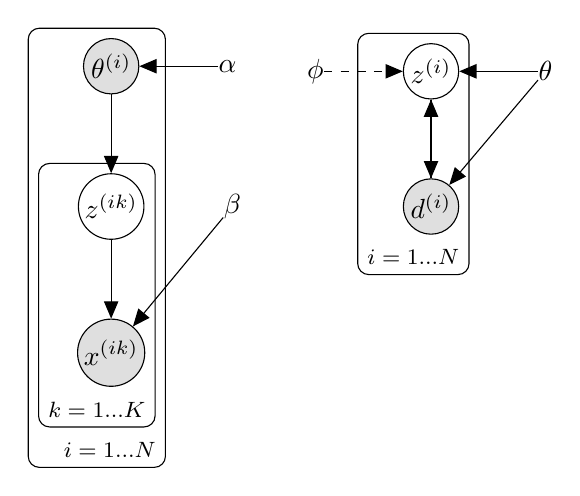
\begin{tikzpicture}[node distance = 1.5cm]
	\node[obs] (x) {$x^{(ik)}$}; 
	
	\node[latent, above=of x] (z) {$z^{(ik)}$}; 
	
	\node[obs, above=of z] (d) {$\theta^{(i)}$}; 
	
	\node[const, right=of d] (a) {$\alpha$} ;
	\node[const, right=of z] (th) {$\beta$} ;
	
	\edge {a} {d};
	\edge {z} {x};
	\edge {d} {z};
	\edge {th} {x};
	
	
	\plate {xz} {(x)(z)} {$k = 1...K$};
	\plate {xzd} {(x)(z)(d)(xz)} {$i = 1...N$};
	
	
	
	\node[const, right=of th] (extra) {};
	\node[obs, right=of extra] (d2) {$d^{(i)}$};
	
	\node[latent, above=of d2] (z2) {$z^{(i)}$};
	
	\node[const, right=of z2] (th2) {$\theta$} ;
	\node[const, left=of z2] (ph2) {$\phi$};
	
	
	\edge {z2} {d2};
	\edge {th2} {z2};
	\edge {th2} {d2};
	\edge [dashed,bend left] {d2} {z2}
	\edge [dashed] {ph2} {z2}
	
	
	
	\plate {zd2} {(z2)(d2)} {$i = 1...N$};
	
	
	\end{tikzpicture}
	\caption{Graphical Model of LDA (left) and VAE Topic Model (left)}
\end{figure}

\subsection{Neural Variational Inference for Topic Models}\label{NVItopic}
NVI Topic Models: discuss in background? Our methods do not depend on this. Could move to discussion? Main contribution is that they got dirichlet  prior to work with laplace approximation.




\chapter{SGVB Topic Models}
In this Chapter, we present in detail the models and methods we use in our experiments. 

\section{Topic VAE}\label{TopicVAE}

In this section we describe our initial approach for topic modeling with SGVB. It closely resembles the VAE model used in the experiments by Kingma and Welling\cite{kingma2013auto}, so we call this a Topic VAE. We will describe the application-specific choices made within the general SGVB framework as described in section \ref{sgvb_section}, and derive the objective function used for optimization. 

\subsection{Model Specifics}

Within the general SGVB framework described in the previous chapter, we specify the following characteristics of our VAE Topic model:

\begin{enumerate}
	\item The representation of our documents $\mathbf{X}$
	\item The encoder $q(\mathbf{z}|\mathbf{x})$
	\item $p(z)$, a prior  over the latent variables
	\item A differentiable way of sampling $\mathbf{z}$ from $p(\mathbf{z}|\mathbf{x})$. 
	\item The decoder $p(\mathbf{x}|\mathbf{z})$
\end{enumerate}

The Bag-of-Words representation of the documents ${\mathbf{X}}$ is normalized such that each document $\mathbf{x}_i$ is represented by a unit vector $\hat{\mathbf{x}_i} = \frac{\mathbf{x}_i}{\sum_{k=1}^{V}x_{ik}}$. Although normalizing data is standard practice in neural network approaches (e.g. \cite{bishop1995neural}), typically each feature is normalized independently to have zero mean and unit variance. In our approach, however, all features (word counts) of a data point (document) are normalized s.t. they represent word probabilities.  Note that this representation no longer contains information on the length of documents, so this approach assumes the latent representations are independent of document length.
\\
The encoder $q(\mathbf{z}|\mathbf{x})$ is a fully connected neural network with one or more hidden layers with ReLU activation functions. The input is $\tilde{\mathbf{x}}$ and the output is the mean and log standard deviation \{$\boldsymbol{\mu}, \log \boldsymbol{\sigma} ^2\}$ of the Multivariate Gaussian $N(\boldsymbol{\mu}, \boldsymbol{\sigma} ^2\textbf{I})$. For one hidden layer this would be the following function:
\begin{align}
\mathbf{h_{e1}} = \text{ReLU}(\mathbf{\hat{x}}\mathbf{W_{e1}} + \mathbf{b}) \label{he1}\\
\boldsymbol{\mu} = \mathbf{h_{e1}W}_{\mu} \label{vae_encoding_mu} \\
\log \boldsymbol{\sigma}^2 = \mathbf{h_{e1}W}_{\sigma} \label{vae_encoding_sig}
\end{align} 


Our encoder therefore only differs from the encoder used in the experiments in Kingma \& Welling \cite{kingma2013auto} in the use of the ReLU function and, in some cases, multiple hidden layers. The ReLU function is slightly faster and preliminary experiments did not show any difference in performance between using ReLU, sigmoid, or tanh nonlinearities. We also use the same prior over latent variables, $p(\mathbf{z}) = N(0,\textbf{I})$ and the same (differentiable) sampling method as in \cite{kingma2013auto}: transformation function $g_\phi(\boldsymbol{\epsilon},\mathbf{x}) = \boldsymbol{\mu} + \boldsymbol{\sigma}^2\odot \boldsymbol{\epsilon}$, and sampling function $p(\epsilon) = N(0,\textbf{I})$. \\
The decoder $p(\mathbf{x}|\mathbf{z})$ is also a neural network with as input (a sample from) latent representation $\mathbf{z}$ and as output the probabilities of a Multinomial distribution, with a ReLU activation function used in each hidden layer. With one hidden layer, this is specified by:

\begin{align}
\mathbf{h_{d1}} = \text{ReLU}(\mathbf{zW_{d1}+b_{d1}})
\\
p(\mathbf{x}|\mathbf{z}) = \text{softmax} (\mathbf{h_{d1}W_{d2}}+\mathbf{b_{d2}})
\end{align}
Where the $\text{softmax}(\mathbf{x}) = \dfrac{e^{\mathbf{x}}}{\sum_{k=1}^{K}e^{x_k}}$


\subsection{Objective Function}
The general form of the SGVB estimator is:

\begin{align}
\tilde{\mathcal{L}}(\boldsymbol{\theta}, \boldsymbol{\phi}, \mathbf{x_i}) = -D_{KL}(q_\phi (\mathbf{z}|\mathbf{x}_i)||p_\theta(\mathbf{z}))  + \frac{1}{L}\sum_{l=1}^{L}\log p_\theta(\mathbf{x}_i|\mathbf{z}_i^{(l)})
\end{align}

And because we consistently only use one sample from sampling function $p(\boldsymbol{\epsilon})$ per data point, this simplifies to:

\begin{align}\label{lb_summary}
\tilde{\mathcal{L}}(\boldsymbol{\theta}, \boldsymbol{\phi}, \mathbf{x_i}) = -D_{KL}(q_\phi (\mathbf{z}|\mathbf{x}_i)||p(_\theta(\mathbf{z}))  + \log p_\theta(\mathbf{x}_i|\mathbf{z}_i)
\end{align}

Because we use Gaussian latent variables with diagonal covariance, we can integrate the KL Divergence analytically as done in Kingma and Welling \cite{kingma2013auto}. Adding the expression for the Multinomial likelihood $p_\theta(\mathbf{x}_i|\mathbf{z}_i)$, we then have
\begin{align}\label{LBest}
\tilde{\mathcal{L}}(\boldsymbol{\theta}, \boldsymbol{\phi}, \mathbf{x_i}) = - \frac{1}{2}\sum\limits_{j=1}^{J}\{1+\log \sigma_{\phi ,ij}^2 - \mu_{\phi,ij}^2 - \sigma_{\phi ,ij}^2\}  + 
\sum_{k=1}^K x_{ik} \log (y_{ik})
\end{align}
\\
Notably, this is the lower bound per \textit{document}. In (bag-of-words) topic modeling, likelihood measures such as perplexity are usually per-word measures. To obtain a per-word lower bound, we must divide the total lower bound for a set of evaluated documents by the number of words in that set: 
\begin{align}\label{perwordLBest}
\tilde{\mathcal{L}_w}(\boldsymbol{\theta}, \boldsymbol{\phi}, \mathbf{X}) = \frac{1}{\sum\limits_{i=1}^{N}\sum\limits_{k=1}^{K}\mathbf{X}_{ik}}\sum\limits_{i=1}^N \tilde{\mathcal{L}}(\boldsymbol{\theta}, \boldsymbol{\phi}, \mathbf{x_i})
\end{align}

We cannot compare this lower bound estimate in \ref{perwordLBest} nor the one in \ref{LBest} directly to different models or evaluation measures. Therefore, the lower bound estimate is merely for model optimization and comparison between Topic VAE models. Although \ref{LBest} and \ref{perwordLBest} are functionally equivalent, a per-word lower bound is independent of average document size and more relatable to other per-word measures in topic modeling, so we use this measure for reporting experimental results.



\section{Stick-Breaking Topic VAE}
No we have described in detail our basic approach to Topic modeling with SGVB, in this section we will describe an alternative to using a Gaussian latent variables; latent variables with Stick-Breaking priors. Where Section \ref{TopicVAE} essentially detailed how to use a VAE for topic modeling, this section details how to use a stick-breaking VAE for Topic Modeling (see \cite{nalisnick2016deep}), and we therefore call this a Stick-Breaking Topic VAE.\\

As in section \ref{TopicVAE}, we will first describe the model specifics and then explain the resulting objective function.
\subsection{Model Specifics}
Once again, for a fully specified model, we need to define:
\begin{enumerate}
	\item The representation of our documents $\mathbf{X}$
	\item The encoder $q(\mathbf{z}|\mathbf{x})$.
	\item $p(\mathbf{z})$, a prior  over the latent variables. 
	\item A differentiable way of sampling $\mathbf{z}$ from $p(\mathbf{z}|\mathbf{x})$. As detailed in \ref{kum}, we can do this by sampling from the inverse CDF of the Kumaraswami distribution: $\mathbf{x} = (1-\boldsymbol{\epsilon}^{\frac{1}{\mathbf{b}}})^{\frac{1}{\mathbf{a}}}$, where $\boldsymbol{\epsilon} \sim \text{Uniform}(0,1)$
	\item The decoder $p(\mathbf{x}|\mathbf{z})$. This remains unchanged te decoder described in section \ref{TopicVAE}.
\end{enumerate}

Most definitions are the same or analogous to a Topic VAE, with the

\begin{enumerate}
	\item Our representation  $\tilde{\mathbf{X}} $ is the same as in for the Topic VAE discussed in \ref{TopicVAE}.
	\item The encoder $q(z|x)$ now encodes the parameters {a, b} of a Kumaraswami distributions
	instead of µ and σ
	2 of univariate Gaussians (see 3.2 and 3.3)
	\item The prior $p(\mathbf{z})$ is now defined by the stick-breaking process described in \ref{sb_process}. Note that in order to do this, we much choose a Dirichlet prior $\alpha_0$. \textit{explain why and how this is a Dirichlet prior, see 2.2 of sbvae paper}
	\item A differentiable way of sampling $\mathbf{z}$ from $p(\mathbf{z}|\mathbf{x})$ is sampling from the inverse CDF of the Kumaraswami distribution: $\mathbf{x} = (1-\boldsymbol{\epsilon}^{\frac{1}{\mathbf{b}}})^{\frac{1}{\mathbf{a}}}$, where $\boldsymbol{\epsilon} \sim \text{Uniform}(0,1)$ (see also \ref{kum})
	\item The decoder $p(\mathbf{x}|\mathbf{z})$ remains unchanged te decoder with a softmax output described in section \ref{TopicVAE}.
\end{enumerate}

\subsection{Objective Function}
The objective function for our Stick-Breaking Topic VAE once again consists of two parts: the KL divergence $D_{KL}(q_\phi (\mathbf{z}|\mathbf{x}_i)||p(_\theta(\mathbf{z}))$ and the reconstruction error $ p_\theta(\mathbf{x_i}|\mathbf{z_i})$ (see equation \ref{lb_summary}). As $ p_\theta(\mathbf{x_i}|\mathbf{z_i})$ is once again modeled as a Multinomial, that part remains unchanged:
$p_\theta(\mathbf{x_i}|\mathbf{z_i}) = \sum_{k=1}^K x_{ik} \log (y_{ik})$. $D_{KL}(q_\phi (\mathbf{z}|\mathbf{x}_i)||p(_\theta(\mathbf{z}))$ is now the KL divergence between the Dirichlet stick-breaking prior distribution and the Kumaraswami posterior distribution. Following Nalisnick \& Smyth \cite{nalisnick2016deep}:

\begin{align}\label{KLSB}
D_{KL}(q(\mathbf{\mathbf{\pi}_i}|\mathbf{x}_i)||p(\mathbf{\pi}_i;\alpha_0)) = \sum_{k=1}^{K}\mathbb{E}_q [\log q(v_{i,k})] - \mathbb{E}_q \log p(v_{i,k})]
\end{align}

We also truncate the infinite-dimensional distribution (stick-breaking process) by setting $\pi_{i,K}$ such that $\sum_{k=1}^{K}\pi_{i,k} = 1$, in which case the KL divergence \ref{KLSB} can be written as:

\begin{align}\label{SBKLFull}
\sum_{k=1}^{K}\mathbb{E}_q [\log q(v_{i,k})] - \mathbb{E}_q \log p(v_{i,k})] = \frac{a_0 -\alpha}{a_0}(-e-\Psi(b_\phi-\frac{1}{b_\phi}))+ \log(a_\phi b_\phi) + \log B(\alpha, \beta) \\
- \frac{b_\phi -1}{b_\phi} 
+ (\beta-1)b_\phi\sum_{m=1}^{\infty}\frac{1}{m+a_\phi b_\phi}B(\frac{m}{a_\phi},b_\phi)
\end{align}

where $e$ is Euler’s constant, $\Psi(\cdot)$ is the Digamma function, and $B(\cdot)$ is the Beta function.
The infinite sum, which originates from a Taylor approximation, is approximated by the leading ten terms as in Nalisnick \& Smith \cite{nalisnick2016deep}. The Digamma function $\Psi$ in \ref{SBKLFull} is approximated with a second order Taylor approximation as higher orders lead to more numerical instability around $b_\phi = 0$. \\
For a full derivation of the KL Divergence between the Kumaraswami distribution and the Dirichlet distribution, see Nalisnick and Smyth (2016) \cite{nalisnick2016deep}.




\section{Dealing with large vocabulary sizes}
One problem of using a VAE approach to topic modeling is the large dimensionality of large corpora. Calculating $p(\mathbf{x}|\mathbf{z})$ dominates the computational cost of each forward pass, and this scales linearly with the vocabulary size. Another reason large vocabulary sizes are troublesome is that very infrequent words get assigned extremely low probabilities and few examples, which respectively lead to numerical instability and overfitting. Typically, only words that occur more often than some threshold in the dataset are used in Topic Modeling. For our approach, this threshold is relatively high for large datasets (see \ref{datasets}). This makes training time and model evaluation a lot faster, and optimization easier. 
Because modeling only the more frequent words has many advantages in our approach, we investigate how to include information on the discarded words in our VAE approach in an efficient, scalable manner.
\\
We project the infrequent words linearly onto a smaller subspace, retaining as much information as possible, and use this as additional information in our encoder. We select from dataset $\mathbf{X}$ a subset of frequent words $\mathbf{X}_{fr}$ to use in the VAE approach described in section \ref{TopicVAE}. Instead of discarding the infrequent words $\mathbf{X}^{if}$, we construct a lower dimensional representation of $\mathbf{X}^{if}$, which we will call $\mathbf{X}^{ld}$. This representation is concatenated with the first hidden layer $\mathbf{h_{e1}}$ (equation \ref{he1} in chapter \ref{TopicVAE}). This way, the second layer of the encoder becomes:
\begin{align}
\mathbf{h_{e2}} = \text{ReLU}(\left(\begin{matrix}
\mathbf{h_{e1}} &
\mathbf{x}^{ld}
\end{matrix}\right)\mathbf{W_{e2}} + \mathbf{b_{e2}}) \label{he1_RP}
\end{align}

This way, the last rows of $\mathbf{W_{e2}}$ multiply only with $\mathbf{x}^{ld}$, yet each hidden unit in $\mathbf{h_{e2}}$ depends on both $\mathbf{x}^{ld}$ and $\mathbf{h_{e1}}$ (and thus also on $\mathbf{x}^{fr}$). Optionally, a hidden layer with learnable parameters can be applied separately to transform $\mathbf{x}^{ld}$ before the concatenation in equation \ref{he1_RP}. The lowercase $\mathbf{h_{e1}}$ and $\mathbf{x}^{ld}$ means this is formulated for one document, but a formulation in terms of minibatches is exactly the same.\\
It is important to note that we do not attempt to model projected data $\mathbf{X}^{ld}$ explicitly in $p(x|z)$  as its probability distribution has now changed.  It therefore merely provides the encoder with additional information. In this work, we investigate two ways of achieving such a lower dimensional representation. 


\subsection{Random Projection}\label{RP}
One effective way of achieving such a lower dimensional representation of sparse data is by means of a Random Projection, a method frequently used for dimensionality in the context of text (see e.g. \cite{bingham2001random} for a comparison to other dimensionality reduction methods). The method is based on the Johnson-Lindenstrauss lemma \cite{frankl1988johnson}, which states that a linear mapping of a large set of high-dimensional vectors to a much lower dimensionality can approximately preserve distances between vectors. A linear mapping of $N$ sparse vectors of dimension $D$ onto a $K$-dimensional space is done by multiplication of the projection matrix $\mathbf{R}_{D\text{x}K}$:

\begin{align}\label{RPeq}
\mathbf{X}^{ld} = \mathbf{X}_{N\text{x}K} = \mathbf{R}_{D\text{x}K}\mathbf{X}_{N\text{x}D}
\end{align}
Where $\mathbf{X}_{N\text{x}D}$ is our bag-of-words data with $N$ documents and vocabulary size $D$.\\

For the Johnson-Lendenstrauss lemma to hold, the matrix $R$ must be orthogonal. However, a results by Hecht-Nielsen \cite{hecht1994context} states that vectors in high-dimensional spaces are very likely to be close to orthogonal. Often Gaussian distributed random matrices are used, and Bingham  and Mannila \cite{bingham2001random} show experimentally that a high-dimensional random matrix with Gaussian distributed values is close to orthogonal. \\
In this work we shall therefore restrict ourselves to a matrix $\mathbf{R}_{D\text{x}K}$ with entries drawn from $N(0,\sigma^2)$. For efficient optimization, it is best that the entries in $\mathbf{X}^{ld}$ are in approximately the same order of magnitude as $H_{e1}$ (see equation \ref{he1}). Therefore we choose $\sigma$ = $\frac{0.5}{\sqrt{\bar{n}}}$, where $\bar{n}$ is the average document length in the dataset. \\
%Data $\mathbf{X}_{N\text{x}D}$ (with $N$ documents and vocabulary size $D$) is a sparse matrix, to be projected onto $K$-dimensional space through $\mathbf{X}_{N\text{x}K} = \mathbf{R}_{D\text{x}K}\mathbf{X}_{N\text{x}D}$ \\
%The $K$ columns of $\mathbf{R}_{D\text{x}K}$ (\ref{RPeq}) are generally of unit length (see \cite{frankl1988johnson}), and it helps if the are orthonormal, which for our application is of negligible computational cost to do. If we normalize each document s.t. the inputs represent probabilities, we can initialize the weights $R$ and $W_1$ with $N(0,1)$, s.t. each hidden unit will receive input distributed as $N(0,1)$. 

\subsection{Singular Value Decomposition}\label{SVD}
The second method of obtaining a lower dimensional representation of infrequent words $\mathbf{X}^{if}$ is by SVD:

\begin{align}
\mathbf{X}^{if} = \mathbf{U\Sigma V}
\end{align}

We then use $K$ left-singular vectors with the highest singular values as $\mathbf{X}^{ld}$. We then once again use each row of $\mathbf{X}^{ld}$ as in equation \ref{he1_RP}.\\
 Bingham \& Mannila \cite{bingham2001random} performed experiments on dimensionality reduction techniques for text processing. Notably, they calculated the distances of random document pairs before and after dimensionality reduction. Reducing dimensionality with SVD lead to lower differences, but Random Projections also preserved these distances quite well. Documents were normalized to have unit length as in our applications, and the vocabulary size in their experiments was 5000 which is comparable to our vocabulary size (see Section \ref{datasets} on datasets). Performing SVD is slower than using a Random Projection, although this is negligible for our application. In Section \ref{large_voc_size} we experiment with both RP and SVD as methods to obtain $\mathbf{X}^{(ld)}$ in the encoder.


\chapter{Experiments and Results}\label{experiments}
\section{General}
Before we describe our specific experiments, we will describe the datasets used, the general optimization method used in our experiments, and the evaluation metrics reported. 
	\subsection{Datasets}\label{datasets}
	For all methods, we ran experiments on the KOS and New York Times datasets, freely available at UCI\footnote{https://archive.ics.uci.edu/ml/datasets/Bag+of+Words}. Both datasets contain only words that occur more than ten times in the whole dataset. The KOS dataset contains 3430 blog post entries and has a vocabulary size of 6906. The dataset was split into 3330 training documents and 130 test documents. The NY times dataset consists of 300,000 articles from the New York Times and has a vocabulary size of 102,660 words. For the NY Times dataset, we only use words that occur over 3,000 times in the dataset, which are 5319 unique words. For this dataset, a test set of 1,000 documents was used.
	
	\subsection{General Optimization Method}\label{optim_section}
	For all experiments we use the AdaM optimization method \cite{kingma2014adam}) with hyperparameters $\beta_1 = 0.9$ and $\beta_2 = 0.99$. Unless otherwise stated, we used learning rate $\alpha = 0.01$ for the KOS dataset and $\alpha = 0.003$ for NY Times dataset.  We use minibatch size of 50 for the KOS dataset and 200 for NY Times.  \\
	Weights for the first layer were initialized with random samples from $N(0,\text{I})$. initial weights in consecutive layers were drawn from  $N(0,\frac{1}{n})$, where $n$ is the number of input units to the corresponding layer. Biases were initialized at 0.
	\\Lastly, the KL divergence is weighted during training, with the weight linearly increasing from 0 to 1 during the first 100 epochs of training. This is done to avoid local optima dominated by the KL divergence. 	
	
	\subsection{Evaluation}
	Comparison between different Topic VAE models is done by calculating the per-word lower bound estimate $\tilde{\mathcal{L}}_w$ (see equation \ref{perwordLBest}) on the test set. However, we can not compare our models to other methods using this metric. \\
	Evaluating topic models is often done by calculating the perplexity of held out words on the test set (e.g. \cite{blei2003latent, newman2007distributed, ranganath2015deep}). In this work, held-out perplexity is calculated for the test set as in Newman \& Welling \cite{newman2007distributed} by using half the words, randomly sampled, in each document for inference (i.e. calculating $p(\mathbf{z}|\mathbf{x})$ ). Let $\mathbf{x}_{i}^{(s)}$ be the half of document $\mathbf{x}_i$ used for inference, and $\mathbf{x}_{i}^{(u)}$ be the other half of the document, used for evaluation. The average per-word perplexity of the unseen words $\mathbf{X^{(u)}}$ in the test documents $\mathbf{X}$ under the word-probabilities $p(\mathbf{x}^{(u)}|\mathbf{z}^{(s)})$, where $\mathbf{z}^{(s)} \sim p(\mathbf{z}|\mathbf{x}^{(s)})$, is then given by:
	
	
	\begin{align}
	\text{perplexity} =  \frac{1}{\sum\limits_{i=1}^{N}\sum\limits_{k=1}^{K}x_{ik}}\sum\limits_{i=1}^N\sum\limits_{k=1}^{K} \log p(x_{k}|\mathbf{z}_{i}^{(s)})x_{ik}^{(u)}
	\end{align}\\
	
	As this perplexity estimate depends also on the sampled noise $\epsilon$ in the reparametrization, it is stochastic. Whenever we estimate the perplexity of a model in this work, we will evaluate every document ten times with independent samples $\epsilon$ to reduce the variance of this estimate to an acceptable level.
	
	\section{Experiments and Results}
	
	
	\subsection{Optimization and characteristics}\label{exp1}
	
	Here we describe experiments on both datasets described in \ref{datasets} with a Topic VAE (\ref{TopicVAE}) to characterize behavior during optimization and to inspect initial results. \\
	Since we have already defined our model (\ref{TopicVAE}) and optimization method (\ref{optim_section}), we need only to define the architecture, i.e. the number of hidden layers and hidden units in both the encoder and the decoder. Overfitting in de decoder is something to keep in mind, so we roughly follow this guideline proposed by Hinton \cite{hinton2012neural} to prevent overfitting: "(...) estimate how many bits it would take to describe each data-vector if you were using a good model. (...) Then multiply that estimate by the number of training cases and use a number of parameters that is about an order of magnitude smaller." This means we can estimate the number of hidden units in the decoder according to $n_h \sim \frac{N*b}{V \cdot 10}$, where N is number of training cases and b is the number of bits needed. As the perplexity is in the order of $2 \cdot 10^3$ (i.e. in \cite{ranganath2015deep}), the number of bits is approximately $\log_2(2 \cdot 10^3) = 11$ for either dataset. For the KOS dataset we have $n_h \sim = \frac{3330 \cdot 11}{6906\cdot 10} = 0.53$. Therefore, we chose to use a linear decoder (i.e. no hidden layer) and 8 latent variables. For the encoder, we use 200 hidden units. Note that even then we use more parameters than ideal and we might be prone to overfitting in the decoder. \\
	We use 100.000 randomly selected documents for training from the NY Times dataset, which means we can use in the order of $n_h \sim = \frac{100.000 \cdot 11}{5319\cdot 10} = 20.7$ hidden units. We use 50 hidden units in the decoder, which might just be enough to overfit, and 400 hidden units in the encoder. We use 32 latent variables for the NY Times dataset. \\
	We evaluate and report the per-word lower bound $\tilde{\mathcal{L}}_w$ on both the train and test set during training, see Figure \ref{lb_first}. The lower bound on the test set does not decrease as the models converge, so they do not overfit on the train set. Notably, the train and test lower bound diverge much more on the KOS dataset than on the NY Times dataset, indicating the model trained on KOS learns much more that is specific to the training set. Because the training set of KOS is so small compared to the NY Times dataset, the model trained on KOS learns more that is specific to the train set and does not generalize as well as the model trained on NY Times. \\
	The 50\% held-out test set perplexity for both models is shown in Figure \ref{perp_first}. Notably, the perplexity does not improve after 50 (NY Times) and 100 (KOS) epochs, where the test lower bounds in Figure \ref{lb_first} start to converge but still show significant improvements after this point. This observation relates to the results of our comparison to other methods (see \ref{comp_other}), and will be discussed further in that section.
	
	\begin{figure}
		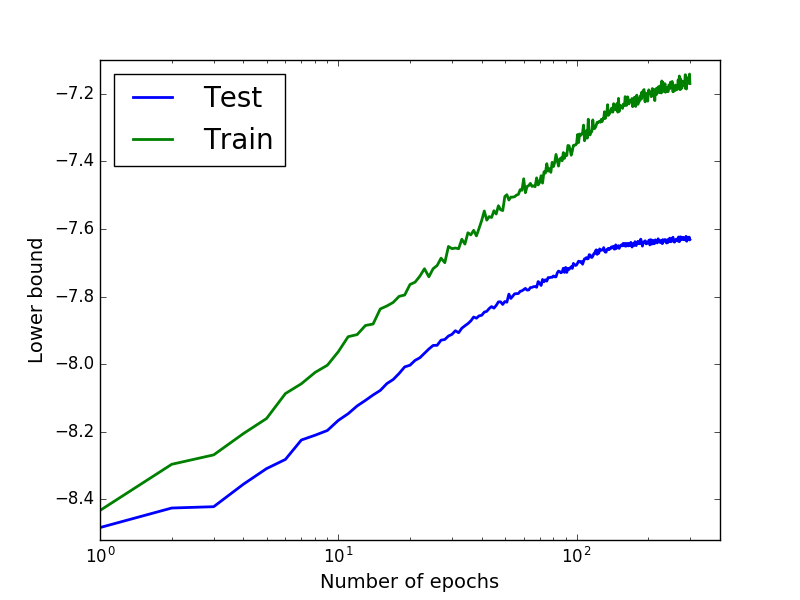
\includegraphics[scale = 0.40]{img/kos_400_0_lb.png}
		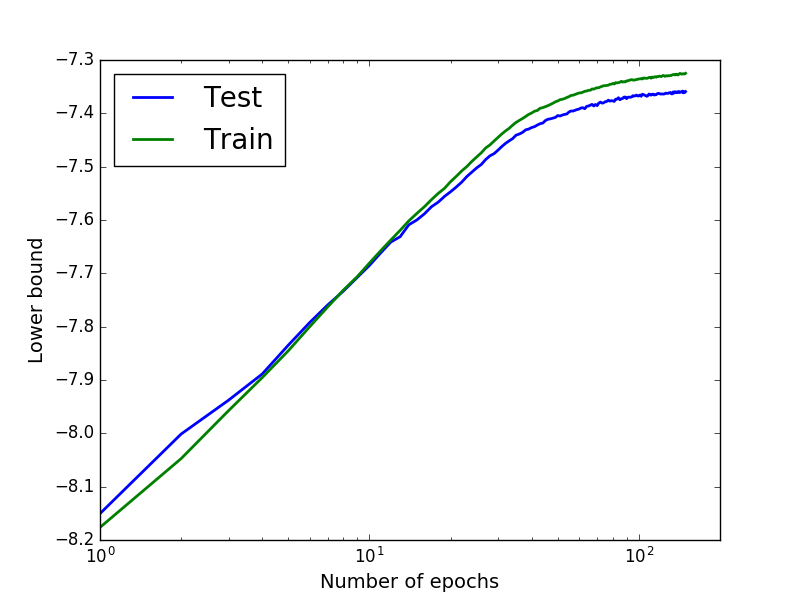
\includegraphics[scale = 0.40]{img/ny_400_50_lb.png}
		\caption{Test and train lower bound evaluated during training. Left: KOS dataset, right: NY Times dataset.}
		\label{lb_first}
	\end{figure}
	
	
	\begin{figure}
		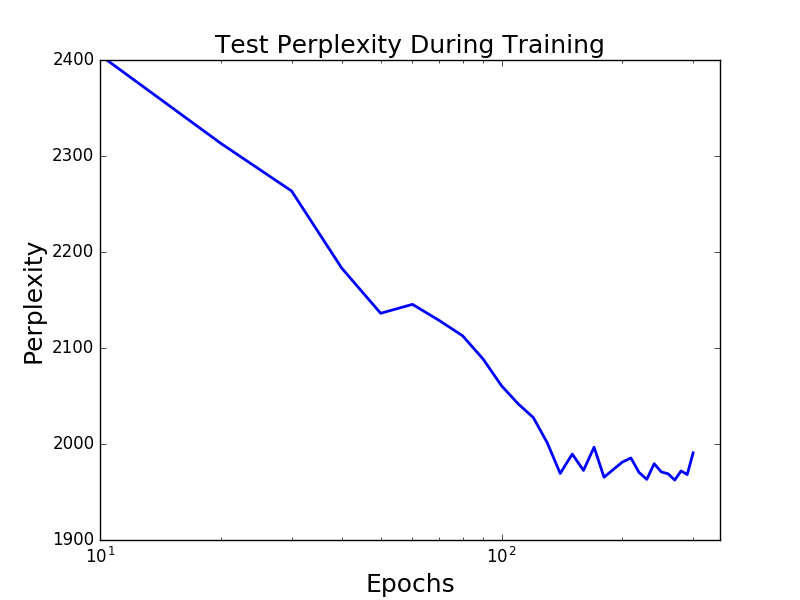
\includegraphics[scale = 0.40]{img/kos_200_0_perp.png}
		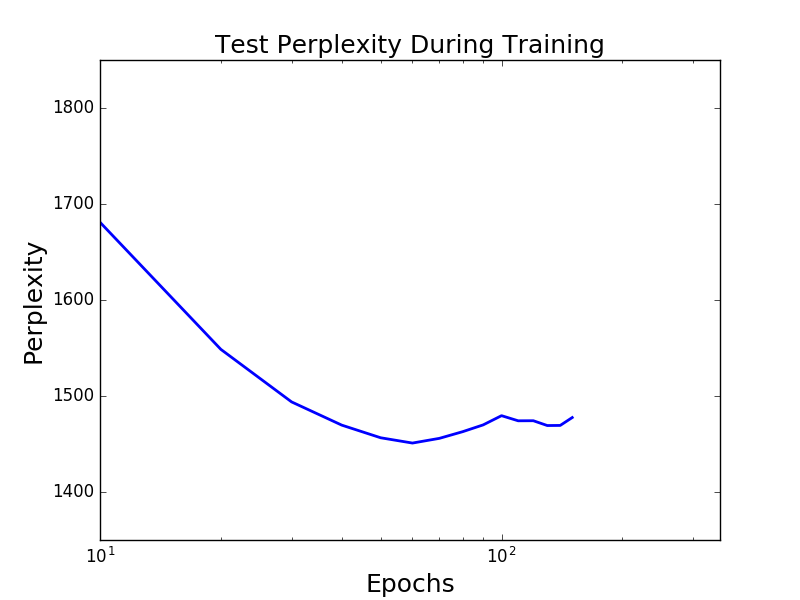
\includegraphics[scale = 0.40]{img/ny_400_50_perp.png}
		\caption{Perplexity evaluated during training. Left: KOS dataset, right: NY Times dataset.}
		\label{perp_first}
	\end{figure}
	
	
	\subsection{Hyperparameter optimization}\label{HO_section}
	Next, we train Topic VAE models with different encoder and decoder structures and compare results. We use 8 and 32 latent variables for the KOS and NY Times datasets, respectively. We use the datasets as specified in \ref{datasets}, but only use 100,000 NY Times documents for training due to limited computational resources. Many other hyperparameters  are the same for all models compared in this experiment and are chosen based on preliminary experiments. These include the optimization method and details, initialization of parameters, gradual increase of KL Divergence (see \ref{optim_section}), but also the use of ReLUs and strength of prior on $p(\mathbf{z}$) (i.e., the variance $\sigma^2$ of the Gaussian $N(0,\mathbf{I})$). We do not vary these because we did not note a significant influence of these choices on model performance in these preliminary experiments. \\
	Figure \ref{HO_KOS} and \ref{HO_NY} detail the lower bound of both the train and test sets of the used datasets for converged models with different encoder/decoder structures. We also report the the 50\% held-out perplexity on the test set.\\
	The results on the KOS dataset are dominated by the tendency of the decoder to overfit. The number of parameters in the decoder is dominated by the last layer, which contains $(n_h \text{ x } V)$ parameters. For the KOS dataset the number of documents $N$ (3300 in the train set) is small compared to the output space $V$ (6906). For the NY Times dataset, with $N = 100,000$ documents used for training and $V = 5319$, this does not become a problem within the used range of architectures.  
		
	\begin{figure}\caption{Hyperparameter Optimization results on KOS. The best scores are shown in red.}
		\centering
			\begin{tabular}{l l|l l |l l }\label{HO_KOS} 		
				Encoder & Decoder & LB Train & LB Test & Perplexity  	\\
				\hline
				200 & -		& -7.142 & \color{red} -7.622 & \color{red} -1990 \\
				
				200 & 20	& -7.062 & -7.740 & 2272 \\
				
				200 & 50	& \color{red} -6.905 & -7.850 & 2554 \\
				
				200-100 & -	& -7.146 & -7.630 & 1992 \\
				
				200-100 & 20	& -7.262 & -7.682 & 2133 \\
				
				200-100 & 50	& -6.941 & -7.789 & 2409 \\
				
				200-100 & 10-10	& -7.217 & -7.737 & 2259 \\
				
				200-100 & 20-20	& -7.121 & -7.872 & 2667 \\
				
				200-100 & 50-50	& -7.024 & -7.961 & 2955 \\
				
			\end{tabular}
		\end{figure}	
		
		\begin{figure}\caption{Hyperparameter Optimization results on NY Times. The best scores are shown in red.}
			\centering
			\begin{tabular}{l l|l l |l l }\label{HO_NY} 		
				Encoder & Decoder & LB Train & LB Test & Perplexity  	\\
				\hline
				400 & -		& -7.354 & -7.379 & 1492 \\
				
				400 & 50	& -7.325 & -7.358 & 1478 \\
				
				1000 & -	& -7.341 & -7.379 & 1513 \\
				
				400-200 & -	& -7.345 & -7.375 & 1493 \\
				
				400-200 & 100	& -7.284 & -7.327 & 1429 \\
				
				1000-600-300 & 200	& -7.212 & -7.308 & 1415 \\
				
				1000-600-300 & 500	& -7.180 & \color{red}-7.297 & \color{red}1384 \\
				
				1000-600-300 & 200-500	& \color{red} -7.161 & -7.324 & 1448 \\
				
			\end{tabular}
		\end{figure}	
		
	
	
	\subsection{Varying the training set size}
	One question regarding our approach is how well this is suited for different amounts of available data. We assume it to be applicable to, and effective for, large amounts of training data. Therefore we want to know if and how much a model improves, in general, when trained on more data. It is also useful to gain some insight in how prone a model is to overfitting with different amounts of data.\\
	To that end, we train a model with a relatively high capacity that was shown to perform well in the results of the hyperparameter optimization experiments in section \ref{HO_section}. We use training set sizes between 5,000 and 300,000 documents and test the models on the same test set of 1,000 documents. We compare effectiveness of converged models by reporting the test lower bound and 50\% held-out test set perplexity. Due to the large difference in training set size, a different number of epochs is used for each model. The results are shown in Figure \ref{increase}. \\
	Convergence took around 100 epochs for all dataset sizes. The linear increase of the KL divergence during the first 100 epochs (see section \ref{optim_section}) prevented earlier convergence for larger amounts of data.   Inspection of the lower bound on the test set revealed that overfitting occurred when using 5,000 and 10,000 training documents, but not when using 20,000 or more documents. This indicates that for larger amounts of data, a more powerful model (i.e. with more parameters) would yield better results. This is also indicated by the fact that the lower bound on the train set does not improve further when using more documents, but the lower bound on the test set does. In Table \ref{HO_NY}, it can indeed be seen that 500 hidden units in the decoder leads to better results than the 200 units used in this experiment, when using 100,000 training documents.
	
	
	\begin{figure}\label{increase}
		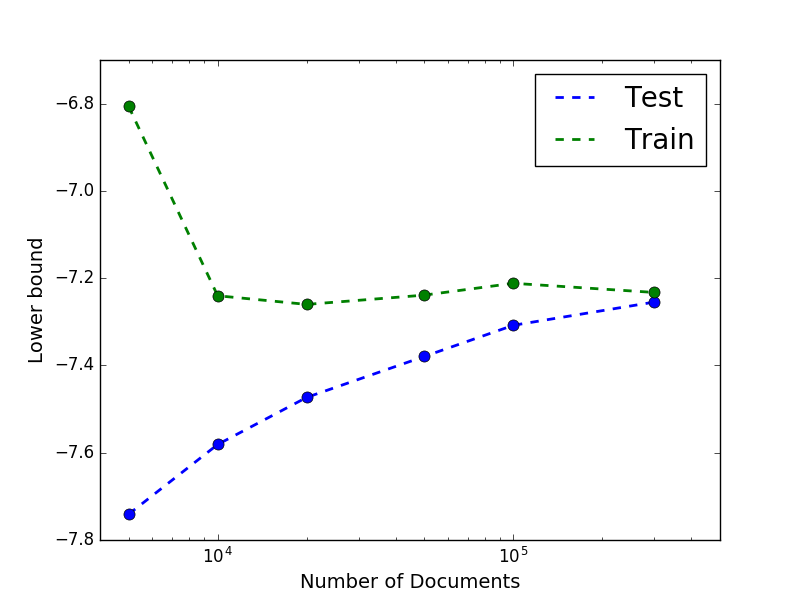
\includegraphics[scale=0.6]{img/increase.png}
		\caption{$\tilde{\mathcal{L}}_w$ evaluated on the train and test set after convergence, for a the model trained on an increasing number of documents.}
	\end{figure}
	
	\subsection{Batch normalization}\label{batch_norm}
	As detailed in \ref{NVItopic}, Srivastava \& Sutton \cite{srivastava2017neural} found that  batch normalization (\cite{srivastava2017neural}), together with a relatively high learning rate and momentum, yielded significantly better results for some model choices they made. \\
	We therefore train a model on each dataset with batch normalization and compare the convergence and model performance to the same model trained without batch normalization. We already use high momentum in our experiments and a learning rate as high as possible without leading to numerical instability (see Section \ref{optim_section}). Srivastrava \& Sutton \cite{srivastava2017neural} found that batch normalization allows for a higher learning rate, so we will once again use the highest learning rate that does not lead to numerical instability.	In our model, we can use batch normalization on each hidden layer activation. Therefore, we choose architectures with multiple hidden layers, trained without batch normalization in section \ref{HO_section}: For the NY Times dataset we use two hidden layers of  400 and 200 hidden units in the encoder and 100 units in the hidden layer of the decoder. For the KOS dataset we used hidden layers of 200 and 100 hidden units in the encoder, but no hidden layer in the decoder.
	Once again we only use the random subset of 100,000 documents for training on the NY Times dataset. \\
	Training the models for a few epochs with different learning rates $\alpha$ showed that the highest $\alpha$ that does not lead to numerical instability is $\alpha = 0.003$ on the NY Times dataset and as high as $\alpha = 0.05$ on the KOS dataset. This was the case both with and without batch normalization. Figure \ref{bn} shows that convergence was not faster with batch normalization. Furthermore, Figure \ref{bn_performance} shows model performance was not significantly different with and without batch normalization. The small differences present are so small they can be attributed to the variance due to (stochastic) optimization and the variance present in the estimate $\tilde{\mathcal{L}}_w$ and the perplexity.
		
	\begin{figure}
		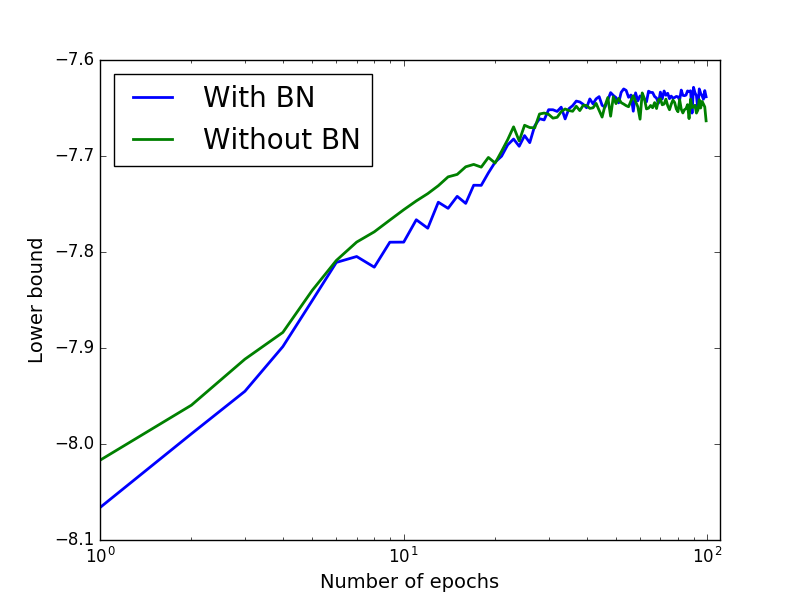
\includegraphics[scale = 0.45]{img/bn_kos_test.png}
		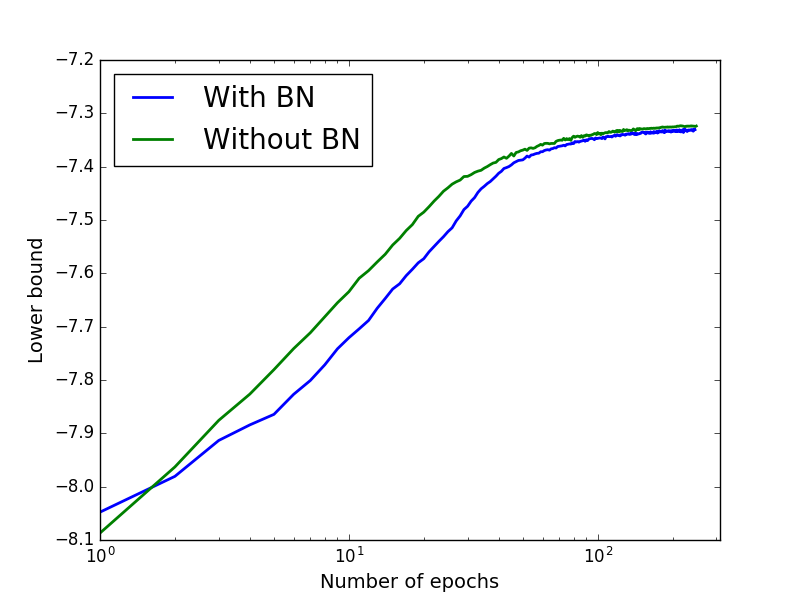
\includegraphics[scale = 0.45]{img/bn_ny_test.png}
		\caption{text}
		\label{bn}
	\end{figure}
		
	\begin{figure}
		\centering
		\begin{tabular}{l|l|l|l }		
			Dataset &  Batch Normalization & Test lower bound & Perplexity  	\\
			\hline
			KOS		 & No	& -7.648 & 1995  \\
			
			KOS 	 & Yes	& -7.638 & 1977  \\ \hline
			NY Times & No	& -7.327 & 1429  \\
			
			NY Times & Yes	& -7.331 & 1449  \\
			
		\end{tabular}
		\caption{Estimates of the lower bound and 50\% held-out test perplexity after convergence with and without batch normalization, on both datasets.}
		\label{bn_performance}
	\end{figure}	
		
		


		
		
		
	\subsection{Stickbreaking Topic VAE}\label{sbvae_exp}
	
	We trained Stickbreaking VAE's (see \ref{sbvae_section}) on both the KOS and NY datasets with an architecture that performed well with Gaussian latent variables. For the NY Times dataset we used 400 and  200 hidden units in the encoder and 100 units in the decoder and 32 latent variables, i.e. we truncated the stick-breaking process at the 32nd latent variable. For KOS we used 400 and 200 hidden units in the encoder and 100 units in the decoder, and 8 latent variables. Optimization of a Stick-Breaking VAE proved to very problematic due to numerical instability. We took the exact same measures to prevent numerical instability in Stick-Breaking VAE's taken by Nalisnick \& Smyth \cite{nalisnick2016deep}: adding small numbers where division by 0 or taking the log of 0 might otherwise occur, and sampling noise $\epsilon$ not from $U(0,1)$ but from $U(0.01, 0.99)$. The the learning rate $\alpha$ was lowered to ten times lower than in our previous experiments, and batch normalization was used on all hidden layers. We tested over a wide range of concentration parameter $\alpha_0$. Despite this, instability was always problematic before convergence. 
	\begin{wrapfigure}{r}{8.5cm}
		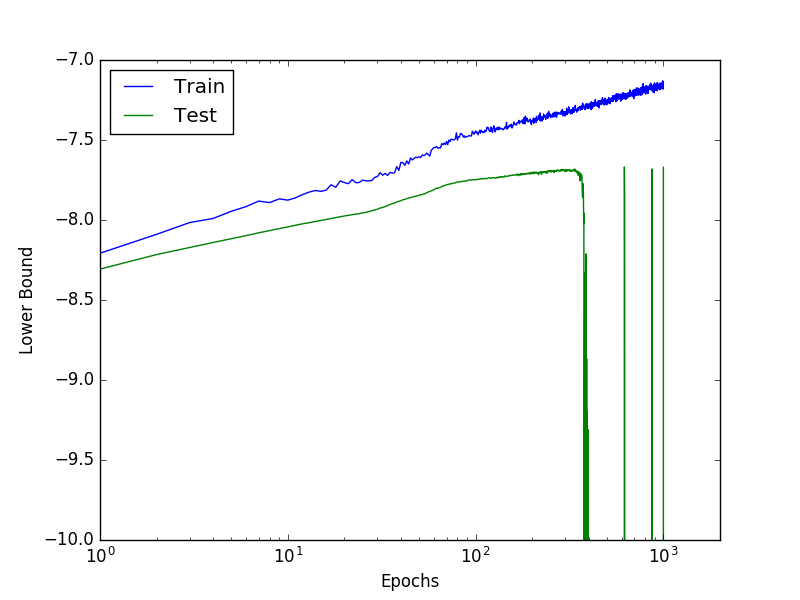
\includegraphics[scale = 0.45]{img/lb_kos_sbvae.png}
		\caption{$\tilde{\mathcal{L}}_w$ during training on KOS dataset.}
		\label{lb_kos_sbvae}
	\end{wrapfigure}
	Figure \ref{lb_kos_sbvae} shows a relatively successful attempt at training a model on the KOS dataset, with only some instability in the evaluation of $\tilde{\mathcal{L}}_w$ on the test set. More often then not, the instability would make training to convergence (or close to it) impossible. Table \ref{sb_res_table} shows the model performance for various values of shape parameter $\alpha_0$ of the prior on the stick-breaking weights $\beta(1,\alpha_0)$. \\
	\begin{figure}%{r}{8.5cm}
		\centering
		\begin{tabular}{l|l|l|l}
			Dataset 	& $\alpha_0$ & Test lb 	& perplexity  \\ \hline
			KOS 		& 0.03		& N/A		&  N/A	\\
			KOS 		& 0.1		& N/A		&  N/A	\\
			KOS 		& 0.3		& -7.9*		&  2551*\\
			KOS 		& 1			& -7.673	&  2085	\\
			KOS 		& 3			& -7.670	&  2058	\\ \hline
			NY Times 	& 0.03		& N/A		& N/A	\\
			NY Times 	& 0.1		& N/A		& N/A	\\
			NY Times 	& 0.3		& -7.503*	& 1789	\\
			NY Times 	& 1			& -7.357	& 1553	\\
			NY Times 	& 3			& N/A		& N/A	\\
		\end{tabular}
		\caption{Test lowerbound and test set perplexity for various values of $\alpha_0$. An asterisk (*) denotes the model could not be trained to convergence, in which case the best performance achieved is reported. N/A denotes the model could not be trained anywhere near convergence.}
		\label{sb_res_table}
	\end{figure}


	Nalisnick \& Smyth \cite{nalisnick2016deep} also found that optimization of a Stick-breaking VAE is harder than a VAE with Gaussian latent variables because of the necessity to back-propagate errors through the stick-breaking process. As each stick length (i.e. latent variable $z_j$) depends on all previous stick-lengths, this results in coupled gradients \cite{nalisnick2016deep}. That they were able to train models successfully is likely because their data consisted of small images (MNIST and Frey Faces\footnote{Available at http://www.cs.nyu.edu/ ̃roweis/data.html}), which are lower dimensional, much less sparse, and include much more regularity than bag-of-words data. We were only able to obtain results with an $\alpha_0$ relatively close to 1. It seems that a very smooth prior distribution $\text{Beta}(1,\alpha_0)$ on the residual fractions $v$ (see section \ref{sbvae_section}) helps, as $\alpha_0=1$ yields a uniform prior distribution $\text{Beta}(1,1) = U(0,1)$.

	
	\subsection{Large vocabulary sizes}\label{large_voc_size}
	
	
	Here we outline how we tested the benefit of of using the infrequent words in the encoder with either a random projection (see \ref{RP}) or SVD (see \ref{SVD}). We use the same number of hidden layers and hidden units as in the previous section \ref{sbvae_exp}. \\
	So far, we used vocabulary sizes of 6906 (KOS) and 5303 (NY Times), which in case of the KOS dataset was the full vocabulary. Therefore, for this experiment we will use only words that occur 50 times or more in the KOS dataset. This way, we will have 1930 frequent words $X^{fr}$ and 4976 infrequent words $X^{if}$. The NY Times dataset contains the 5319 frequent words (see \ref{datasets}), and 97341 infrequent words which were discarded in all previous experiments. These infrequent words will be represented by either a random projection of these words or the largest singular values, as described in \ref{RP} and \ref{SVD}, respectively. We use dimensionality of the representation of the projection of words $K = 200$ in all experiments. \\
	We use an encoder with a large capacity: three hidden layers of 1,000, 600 and 300 hidden units, respectively. For the decoder we use one hidden layer with 200 units.
	Table \ref{rpsvd_results} compares both methods on both datasets to the baseline where $X^{if}$ is not used. Hardly any improvements over the baseline are realized: Using a hidden layer yields comparable results and not using a hidden layer seems to even have a slight adverse effect on performance compared to the baseline for both datasets. It seems that the information in $X^{if}$ is not very useful to learn a better inference model $p(z|x)$. Another  reason for the poor results might be that, although the capacity of the encoder is very high, the smaller capacity of the decoder is the limiting factor of the models and a better encoding $p(z|x)$ would therefore not lead to a better reconstruction $p(x|z)$.
	
	\begin{figure}
		\centering
		\begin{tabular}{l|l|l|l|l}
			dataset & method & hidden layer & test $\tilde{\mathcal{L}}_w$ & perplexity \\ \hline
			KOS	&	None	& no &	\color{red} -6.639	&	744 \\
			KOS	&	RP	&	no &-6.645	&	735 \\
			KOS&SVD&no &-6.645&742 \\
			KOS	&	RP	&	yes & -6.642	&	\color{red}730 \\
			KOS&SVD&yes &\color{red}-6.639&739 \\ \hline 
			NY Times&None&no & -7.308 & 1415\\
			NY Times&RP&no &-7.349&1470 \\
			NY Times&SVD&no &-7.334&1441 \\ 
			NY Times&RP&yes &-7.310&1401 \\
			NY Times&SVD&yes &\color{red}-7.306&\color{red}1394 \\
		\end{tabular}
		\caption{Results for different methods of using $X^{if}$ in the encoder.}
		\label{rpsvd_results}
	\end{figure}

	\subsection{Overview of investigated methods}\label{comp_methods_details}
	As described in \ref{comp_methods_details}, we compare the results of the different methods used in this thesis on the NY Times dataset: Gaussian (\ref{exp1}) and stick-sreaking (\ref{sbvae_exp} ) latent variables, Random Projections or SVD on infrequent words (\ref{large_voc_size}), and the use of Batch Normalization (\ref{batch_norm}). Figure \ref{comp_ny} compares the test lower bound and 50\% held-out test perplexity for the different methods on two architectures used in the hyperparameter optimization section (section \ref{HO_section}, Table \ref{HO_NY}).\\
	In general, the basic approach without Random Projections or SVD on $X^{if}$ and with Gaussian latent variables was hardly improved upon. Batch normalization did not lead to improvements in convergence speed or model performance, and stick-breaking priors on the latent variables proved very hard to optimize.
	
	\begin{figure}
		\begin{tabular}{l l l l | l l}	
			Architecture* & Latent Variables & Infrequent words & Batch Normalization & Test lower bound & Perplexity  	\\ \hline
			&	Gaussian	&	Unused				&	no	&	-7.320 	& 1429 	\\ 
			&	Gaussian	&	Unused				&	yes  &	-7.331 	& 1449 	\\ 
			S	&	Gaussian	&	Random Projection	&	no	&	-7.380 	&  1500 	\\ 
			&	Gaussian 	&	SVD					& no	&	-7.372 	& 1487	\\ 
			&	stick-breaking	&	Unused	&	yes &	-7.363& 1523			\\  \hline
			
			&	Gaussian	&	Unused				&	no	&	-7.308 	& 1415 	\\ 
			&	Gaussian	&	Unused				&	yes  &	 -7.310	& 1420 			\\ 
			L	&	Gaussian	&	Random Projection	&	no	&	 -7.310	&   1401	\\ 
			&	Gaussian 	&	SVD					& no	&	 \color{red} -7.306	& \color{red} 1394			\\ 
			&	stick-breaking	&	Unused	&	yes & N/A	& 	N/A					\\  \hline
			
		\end{tabular}
		\caption{Overview of model performance of different approaches used for two different architectures. The smaller architecture, denoted with S, has 400 and 200 units in the hidden layers of the encoder and 100 hidden units in the decoder. The larger one, denoted with L, has has 1,000, 600 and 300 units in the hidden layers of the encoder and 200 hidden units in the decoder.}
		\label{comp_ny}
	\end{figure}
	

	
	\subsection{Comparison to Other Methods}\label{comp_other}
	\begin{figure}
		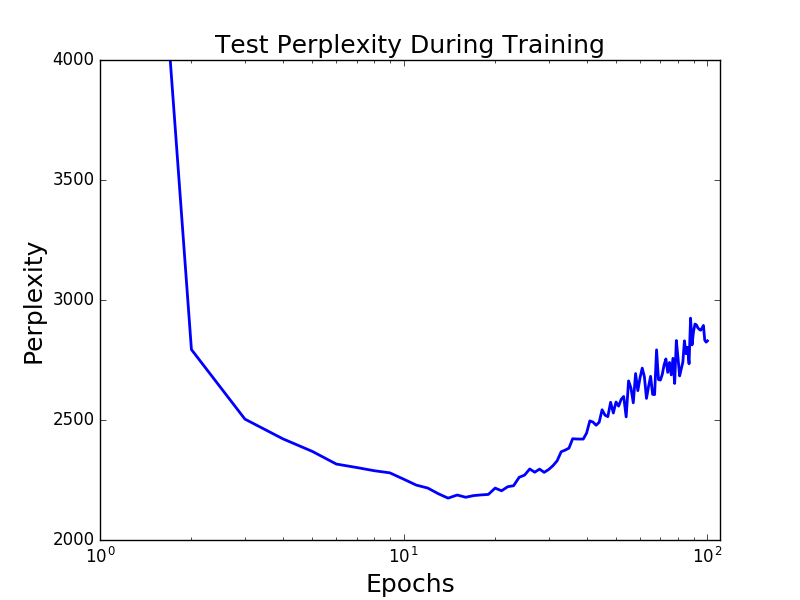
\includegraphics[scale=0.45]{img/10pcperplex.png}
		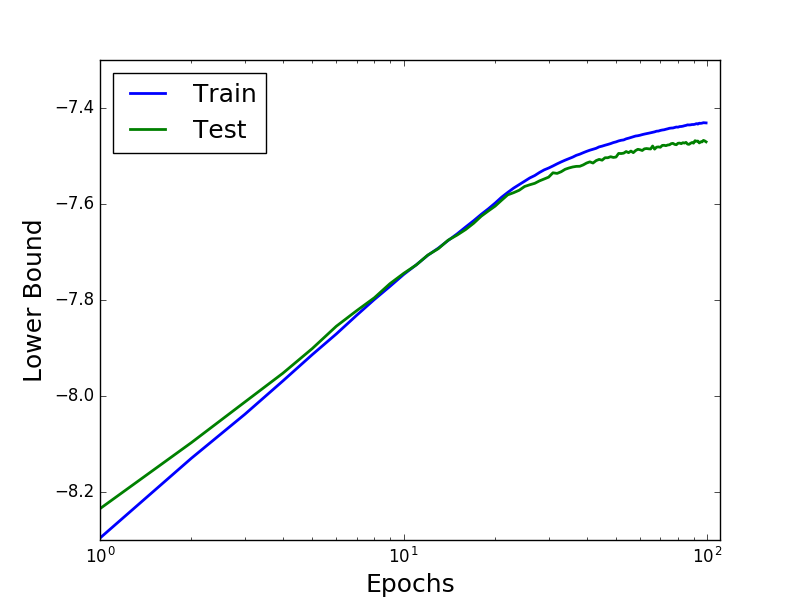
\includegraphics[scale=0.45]{img/lbcompdef.png}
		\caption{10\% held-out test set perplexity and $\tilde{\mathcal{L}}_w$ evaluated during training.}
		\label{10pctoverfit}
	\end{figure}	
	In this section we compare the Topic VAE method to the results on LDA (\cite{blei2003latent} and section \ref{LDA})and Deep Exponential Families (\cite{ranganath2015deep} and section \ref{DEF}) reported in \cite{ranganath2015deep}. 
	LDA is still a polular model and Deep Exponential Families is the state-of-the-art in terms of reported held-out test perplexity. Ranganath et al. \cite{ranganath2015deep} trained models on the 8,000 most frequent words of 165,000 NY Times documents. They report the 10\% held-out test set perplexity on a test set of 1,000 of the same documents. We do the same with a Topic VAE model with Gaussian latent variables and no batch normalization. We use the same architecture referred to as "Large" in Table \ref{comp_ny}. \\
	\begin{wrapfigure}{r}{5cm}
		\bgroup
		\def\arraystretch{1.2}
		\begin{tabular}{||l|l||}
			\hline \hline
			Model	& Perplexity\\ \hline \hline
			LDA	&  2717\\ \hline
			DEF (worst) & 2653 \\ \hline
			DEF (best) & 2251 \\ \hline
			VAE Topic & 2174 \\ \hline
		\end{tabular}
		
		\caption{10\% held-out perplexity on 1,000 held out NY Times documents. Lower is better. LDA was optimized with black box variational inference \cite{ranganath2014black}}
		\egroup
		\label{comp_def}
	\end{wrapfigure}
	An important finding is that during training the perplexity starts getting worse even though the test lower bound has not finished improving.	This is shown in Figure \ref{10pctoverfit}. This observation connects to the earlier observation that in previous experiments, the 50\% held-out test perplexity stopped improving before the model had converged (see Figure \ref{perp_first}). This indicates that held out test perplexity, especially when few words are used for inference, is a bad measure of model performance at least in some cases. To the best of our knowledge, this problem has not been described or investigated in the literature. \\
	To compare our model to the other methods, we therefore use early stopping, i.e. we report the best 10\% held-out test perplexity achieved during training, even though results get worse later on during convergence. As can be seen in Figure \ref{comp_def}, the Topic VAE scores better than the other methods. 

	
	\textit{discuss why this is fair? Discuss implications for comparing DEF to our method with different perplexity? Note that we do not want to run this ourself because computation and time?}. \\
	
	


	




		
\chapter{Conclusion}
In this work we investigated how to best apply SGVB top Topic Modeling. We first ran experiments with a typical VAE approach with a Multinomial reconstruction error. With these experiments, we investigated which architectures work well, how well the model performs with increasing amounts of data, and if the model easily overfits. Next, we developed two possible improvements: A Stick-Breaking VAE and the use of infrequent words in the encoder. We ran experiments with these methods and compared the results to our initial model. We also tested whether batch normalization is a useful inclusion in the developed models. Lastly, we compared our model to LDA and DEF by evaluating the 10 \% held-out perplexity on the NY Times dataset.\\
In our experiments with the Topic VAE, we found that the decoder easily overfits on the small KOS dataset. The decoder did not overfit on the larger collection of NY Times documents; for that dataset, the best results were achieved with a more powerful decoder. For both datasets, additional hidden layers in the encoder did not lead to large improvements. We further determined that batch normalization did not benefit optimization or model performance within the performed experiments. \\
The performance of the Topic VAE improved when trained on increasing amounts of data, as is to be expected. This supports the claim that a Topic VAE is a useful model choice for large datasets.\\
The presented Stick-Breaking Topic VAE did not yield significant improvements over the Topic VAE. The Stick-Breaking VAE could not be trained to convergence due to unsolved numerical stability issues and even  performance similar to the Topic VAE was not achieved. \\
As for the additional use of infrequent words in the encoder of a Topic VAE, this addition only lead to small improvements in performance. We would therefore not recommend using the infrequent words in a dataset at all in practice. \\
While it proved hard to improve over the basic Topic VAE, it outperformed LDA and the state-of-the-art DEF. It was also shown that 10\% held-out test perplexity used to compare methods is not a good measure of model performance in our case, as perplexity decreased during training while the test lower bound decreased. We therefore used early stopping for our method. It is unclear if LDA and DEF would also achieve better 10\% held-out test perplexity scores with early stopping. It would therefore be good to also compare methods on e.g. 50\% held-out test perplexity, which was unfortunately not feasible within this work.\\
Based on this work, a Topic VAE is an excellent model for bag-of-words topic modeling on large collections of text: It is straightforward to train, scales well with large amounts of documents, and achieves state-of-the-art results. 

\section{Future Work}
better comparison, mainly perplexity but perhaps mention\\ topic coherence\\
deeper+dropout\\
multiple layers of latent variables, such as DEF basically has

\bibliography{ref}

	\chapter{Appendix A: Graph Convolutional Networks for Topic VAEs}
	Bag-of-words data can be seen as a bipartite graph between document nodes and word nodes. From this perspective, it makes sense to look into incorporating the work by Kipf \& Welling \cite{kipf2016semi} on Graph Convolutional Networks in our approach. Therefore, as part of this thesis, efforts were made to combine GCNs and Topic VAEs. Ultimately, these efforts did not lead to feasible  model adjustments or improvements and no experiments were conducted. However, in this Appendix we will detail these efforts after briefly introducing GCNs. 

	\section{Graph Convolutional Networks}
	Explain Kipf \& Welling 
	\section{Combining GCNs with Topic VAEs}	
	As stated earlier, the first layer of a GCN is given by:
	\begin{align}\label{GCE_layer}
	H = \text{ReLU}(\bar{D}^{-\frac{1}{2}}\bar{A}\bar{D}^{-\frac{1}{2}}FW)
	\end{align}
	\\
	Where ReLU can be an other nonlinearity of choice. $\bar{A}$ is the (symmetric) adjacency matrix $A$ with added self connections $I$:$\bar{A} = A+I$, and $\bar{D_{ii}}=\sum_j\bar{A}_{ij}$. Further, $W$ is a trainable weight matrix similar to those in our earlier approaches. In our application, $\bar{A}$ would be of dimension $(N_d + V) \text{ x } (N_d + V)$, with both the upper left corner and the bottom right corner an identity matrix (note: explain what $A_{ij}$ is). We can rewrite \ref{GCE_layer} as:
	
	\begin{align}
	H = \text{ReLU}(X'W)
	\end{align}
	
	Where $X' = \bar{D}^{-\frac{1}{2}}\bar{A}\bar{D}^{-\frac{1}{2}}F$. A straightforward way of using Graph Convolutions is to incorporate one (or more) Graph Convolutions in our encoder as in \ref{GCE_layer}. \\ In this case, $F$ would logically reduce to $I$ since we have no node features. \\
	Let us rewrite $X'W$, leaving out the self-connections $\mathbf{I}$ in $\mathbf{A}$: 
	\begin{align}
	X' = \bar{D}^{-\frac{1}{2}}
	\left( \begin{matrix} 
	0 && G \\
	G^T && 0
	\end{matrix} \right) \bar{D}^{-\frac{1}{2}}W = 
	\left(\begin{matrix}
	\bar{G}W_1 \\
	\bar{G^T}W_2
	\end{matrix}\right)\label{highlow}  
	\end{align}
	Where $\bar{G}_{ij} = 
	\frac{G_{ij}}{\sqrt{\sum_i G_{ij} \sum_{j} G_{ij}}}$ 
	
	We now have multiplications with two weight matrices $W_1$ and $W_2$, one that has parameters for each $N_d$ documents and one that has parameters for each word in $V$. Having parameters for each document is not scalable to large datasets, especially since a batched approach to $\bar{G^T}W_2$ is impossible.\\
	One way of encoding some document-level information is to use the covariance matrix $\bar{G^T}\bar{G}$ in stead of $\bar{G^T}$. Now, the number of parameters in our first layer would scale with $(2\cdot V)$ instead of $(V+N)$. \ref{highlow} now becomes:
	\\
	\begin{align}
	\left(\begin{matrix}
	\bar{G}W_1 \\
	\bar{G^T}\bar{G}W_c
	\end{matrix}\right)
	\end{align}
	\\
	Using a minibatch approach to $\bar{G^T}\bar{G}W_2$ requires calculating $\bar{G^T}\bar{G_{batch}}W_c$ for each batch, which is of complexity $O(V\text{ x }V \text{ x } h)$, where $h$ is the number of hidden units. Even for a large batch size, this is much more expensive than calculating the sparse multiplication $\bar{G}_{batch}W_1$, which is of $O(\text{nonzero}(\bar{G}_{batch}) \text{ x } h \text{ x } \text{batchsize})$. 
	\\
	Using the full covariance matrix for each minibatch allows for computing $\bar{G^T}\bar{G}$ only once. However, writing out the first layer for one row $\mathbf{g}$ of $\bar{G}$ shows us this approach does not combine information in $\mathbf{g}$ and $\bar{G}_T\bar{G}$:
	\begin{align}
	h_1 = \text{ReLU}(
	\left(\begin{matrix}
	\mathbf{g} \\
	\bar{G^T}\bar{G}
	\end{matrix}\right)W_1 +b_1)
	\\
	h_1 = 
	\text{ReLU}(\left(\begin{matrix}
	\mathbf{g}W_{1a} \\
	\bar{G^T}\bar{G}W_{1b}
	\end{matrix}\right) + b_1)
	\end{align}
	\\
	Leaving out $\bar{G}^TW_2$ in \ref{highlow} leaves us with the original first layer of our encoder, except with a different TF-IDF-like normalization of our data. \\ While this normalization could be used for a VAE approach, this begs the question how to model $p(\mathbf{x|z})$. While we chose to model $p(\mathbf{x|z})$ as a Multinomial (see Chapter \ref{TopicVAE} and equation \ref{LBest}), the normalized data is no longer Multinomially distributed and there is no obvious choice for modeling $p(\mathbf{x|z})$.\\
	In this Appendix we have investigated the use of a GCN for incorporation in SGVB Topic modeling. We found that it is not possible to incorporate this without adding parameters to the model for each document. This is detrimental to scalability, which is one of the  main advantages of our general approach. Furthermore, we considered augmenting the data pre-training, but this invalidates the Multinomial distribution of the data.
	Therefore, we concluded that GCNs are not useful in combination with SGVB Topic modeling, and did not perform any experiments on this.

\end{document}